\documentclass[11pt]{article}
\usepackage[utf8]{inputenc}
\usepackage[T1]{fontenc} % uses T1 fonts (better quality)
\usepackage{lmodern} % uses Latin Modern fonts
\usepackage[margin=1in]{geometry}
\usepackage[dvipsnames]{xcolor}
\usepackage{ragged2e}
\renewcommand{\baselinestretch}{1.15}
\usepackage{tikz}
\usetikzlibrary{automata,scopes,shapes,matrix,arrows,decorations.pathmorphing}
\tikzset{>={stealth}}
\usepackage{mathtools}
\usepackage{bm}
\usepackage{graphicx}
\usepackage[makeroom]{cancel}
\usepackage{pdfpages}
\usepackage{amssymb}
\usepackage{gensymb}
\usepackage{rotating}
\definecolor{CrispBlue}{HTML}{0176AE}

\begin{document}
\begin{center}
\LARGE{ECE 345 / ME 380: Introduction to Control Systems\\Problem Set \#4}\\[1.5em]
\large David Kirby\\[1.5em]
\large \textbf{Due Tuesday, November 24, 2020 at 3:30pm}\\[2.5em]
\end{center}

\noindent Consider the system in the figure below with \(G(s)=\displaystyle\frac{8}{s^2+4s+8}\).\par
    \begin{figure}[h!]
    \centering
    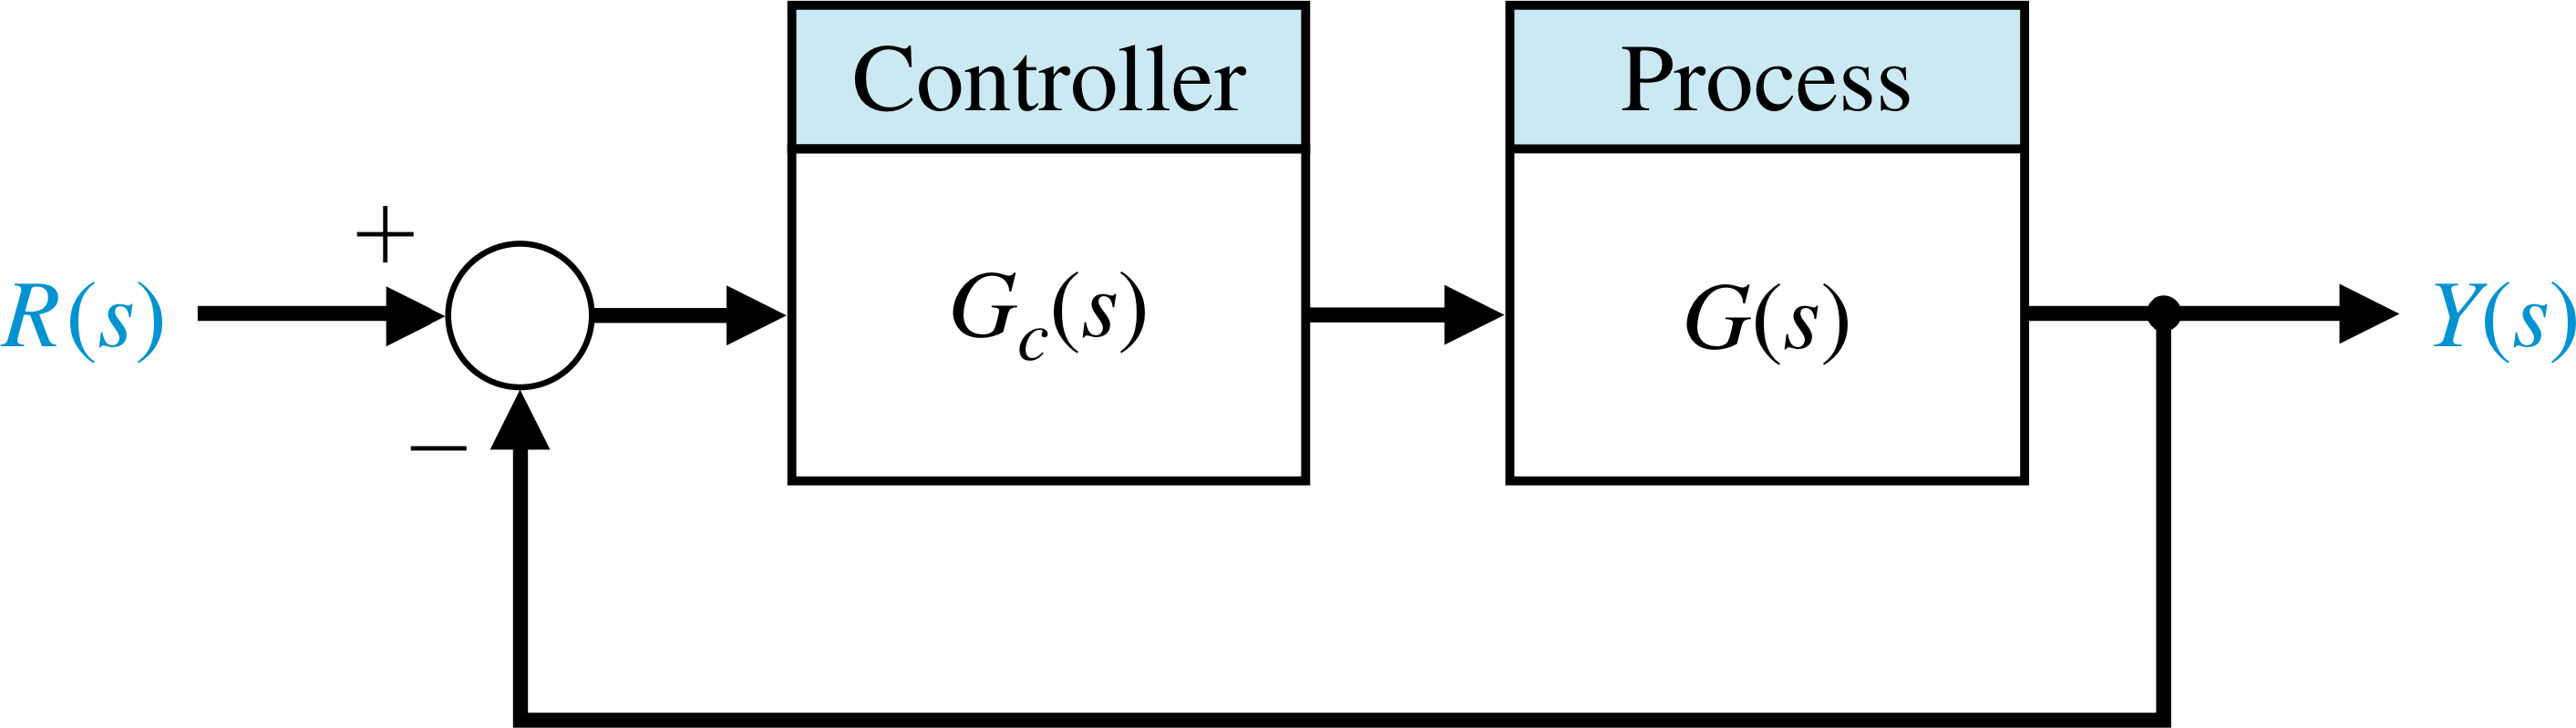
\includegraphics[width=0.55\textwidth]{./Images/Fig05-001.png}
    \end{figure}
\noindent This assignment will investigate the use of three different controllers \(Gc(s)\) under negative unity feedback: (1) Lead \(Gc(s) = K \frac{s+4}{s+10}\), (2) Lag \(Gc(s) = K \frac{s+10}{s+4}\), and (3) PID \(Gc(s) = K \frac{(s+4)(s+10)}{s}\).
\begin{enumerate}
    \item (+10 points) Consider the lead controller \( G(s)=\displaystyle\frac{s+4}{s+10} \).
        \begin{enumerate}
            \item Plot (via Matlab) or sketch (by hand) the root locus for this system. In Matlab, use \texttt{GcG = tf(8*[1 4],conv([1 10],[1 4 8]))} to represent the open-loop system \(G_c(s)G(s)\), then use \texttt{rlocus(GcG)}.\par
                \color{CrispBlue}
                Please see Matlab plot below.
                \color{black}
            \item Using the Hurwitz conditions, find the values of \(K >0\), if any, that will make the closed-loop system asymptotically stable.
                \color{CrispBlue}
                \begin{align*}
                    \Delta_{CL}(s) &= D(s) + K N(s)\\
                    &= (s+10)(s^2+4s+8)+8K(s+4)\\
                    &=s^3+14s^2+(8K+48)s+(32K+80)
                \end{align*}
                \begin{align*}
                    a_0=32K+80, && a_1=8K+48, && a_2=14, && a_3=1
                \end{align*}
                \begin{align*}
                    a_1a_2-a_0>0, && a_2>0,\quad a_1>0,\quad a_0>0\\
                    (8K+48)(14)-(32K+80)>0 && 14>0,\quad 8K+48>0,\quad 32K+80>0\\
                    K>-\frac{37}{5} && K>-6,\quad K>-\frac{5}{2}
                \end{align*}
                Closed-loop system will be stable for all values \(K>0\).
                \color{black}
            \item Use the Matlab command \texttt{margin(GcG)} to compute the phase margin and gain margin with \(K= 1\). Is the system stable with \(K= 1\)?\par
            \color{CrispBlue}
            Please see Matlab plot below. \(P_m = \infty, G_m = \infty\), therefore the system is stable with \(K= 1\).
            \color{black}
        \end{enumerate}
    \item (+15 points) Consider the lag controller \( G(s)=\displaystyle\frac{s+10}{s+4} \).
        \begin{enumerate}
            \item Plot (via Matlab) or sketch (by hand) the root locus for this system. In Matlab, use \texttt{tf} to represent the open-loop system \(G_c(s)G(s)\), then use \texttt{rlocus(GcG)}.\par
            \color{CrispBlue}
            Please see Matlab plot below.
            \color{black}
            \item Using the Hurwitz conditions, find the values of \(K >0\), if any, that will make the closed-loop system asymptotically stable.
                \color{CrispBlue}
                \begin{align*}
                    \Delta_{CL}(s) &= D(s) + K N(s)\\
                    &= (s+4)(s^2+4s+8)+8K(s+10)\\
                    &=s^3+8s^2+(8K+24)s+(80K+32)
                \end{align*}
                \begin{align*}
                    a_0=80K+32, && a_1=8K+24, && a_2=8, && a_3=1
                \end{align*}
                \begin{align*}
                    a_1a_2-a_0>0, && a_2>0,\quad a_1>0,\quad a_0>0\\
                    (8K+24)(8)-(80K+32)>0 && 8>0,\quad 8K+24>0,\quad 80K+32>0\\
                    K<10 && K>-3,\quad K>-\frac{2}{5}
                \end{align*}
                Closed-loop system will be stable for values \(K<10\).
                \color{black}
            \item Use the Matlab command \texttt{margin(GcG)} to compute the phase margin and gain margin with \(K= 1\). Is the system stable with \(K= 1\)?\par
                \color{CrispBlue}
                Please see Matlab plot below. \(P_m = 47.1 \degree , G_m = 20 \text{ dB}\), therefore the system is stable with \(K= 1\).
                \color{black}
            \item What is the gain margin in magnitude (not dB)? Compare this to your answer in Question 2(b).\par
                \color{CrispBlue}
                \( G_m = 20 \log{x}=20 \quad \rightarrow \quad G_m = 10\). We get the same results as in 2(b).
                \color{black}
        \end{enumerate}
    \item (+10 points) Now compare the lead and lag controllers.
        \begin{enumerate}
            \item Compare the order, number of asymptotes, and location of the centroid for the two systems. What is the primary effect of reversing the location of the controller pole and zero?\par
            \color{CrispBlue}
            The order and number of asymptotes are the same for both the lead and the lag controllers; however, the centroids are different. If the pole is greater than the zero, the centroid will stay in the left half plane. Reversing the location, as the zero grows larger than the pole, the centroid is pushed further right and eventually into the right-half plane.
            \color{black}
            \item Which of the two systems (under lead or lag control) has \textit{more} relative stability? Justify your answer in a single sentence.\par
            \color{CrispBlue}
            The lead controller is stable for all \(K>0\), therefore it has more relative stability.
            \color{black}
        \end{enumerate}
    \item (+10 points) Lastly, consider the effect of a Proportional-Integral-Derivative (PID) controller \(Gc(s) = K \displaystyle\frac{(s+4)(s+10)}{s} = 14K + \frac{40K}{s} + Ks\).
        \begin{enumerate}
            \item Plot (via Matlab) the root locus for this system. Use \texttt{tf} to represent the open-loop system \(G_c(s)G(s)\), then use \texttt{rlocus(GcG)}.\par
            \color{CrispBlue}
            Please see Matlab plot below.
            \color{black}
            \item Use \texttt{rlocfind} to find the value of \(K\) that results in a critically damped system.\par
            \color{CrispBlue}
            \(K = 5.1213\)
            \color{black}
            \item Based on your root locus plot, is it possible to destabilize the system by making \(K\) sufficiently large? Why or why not?\par
            \color{CrispBlue}
            The root locus plot shows roots in the left-half plane for \(K>0\), therefore the system will be asymptotically stable for all \(K>0\).
            \color{black}
        \end{enumerate}
\end{enumerate}
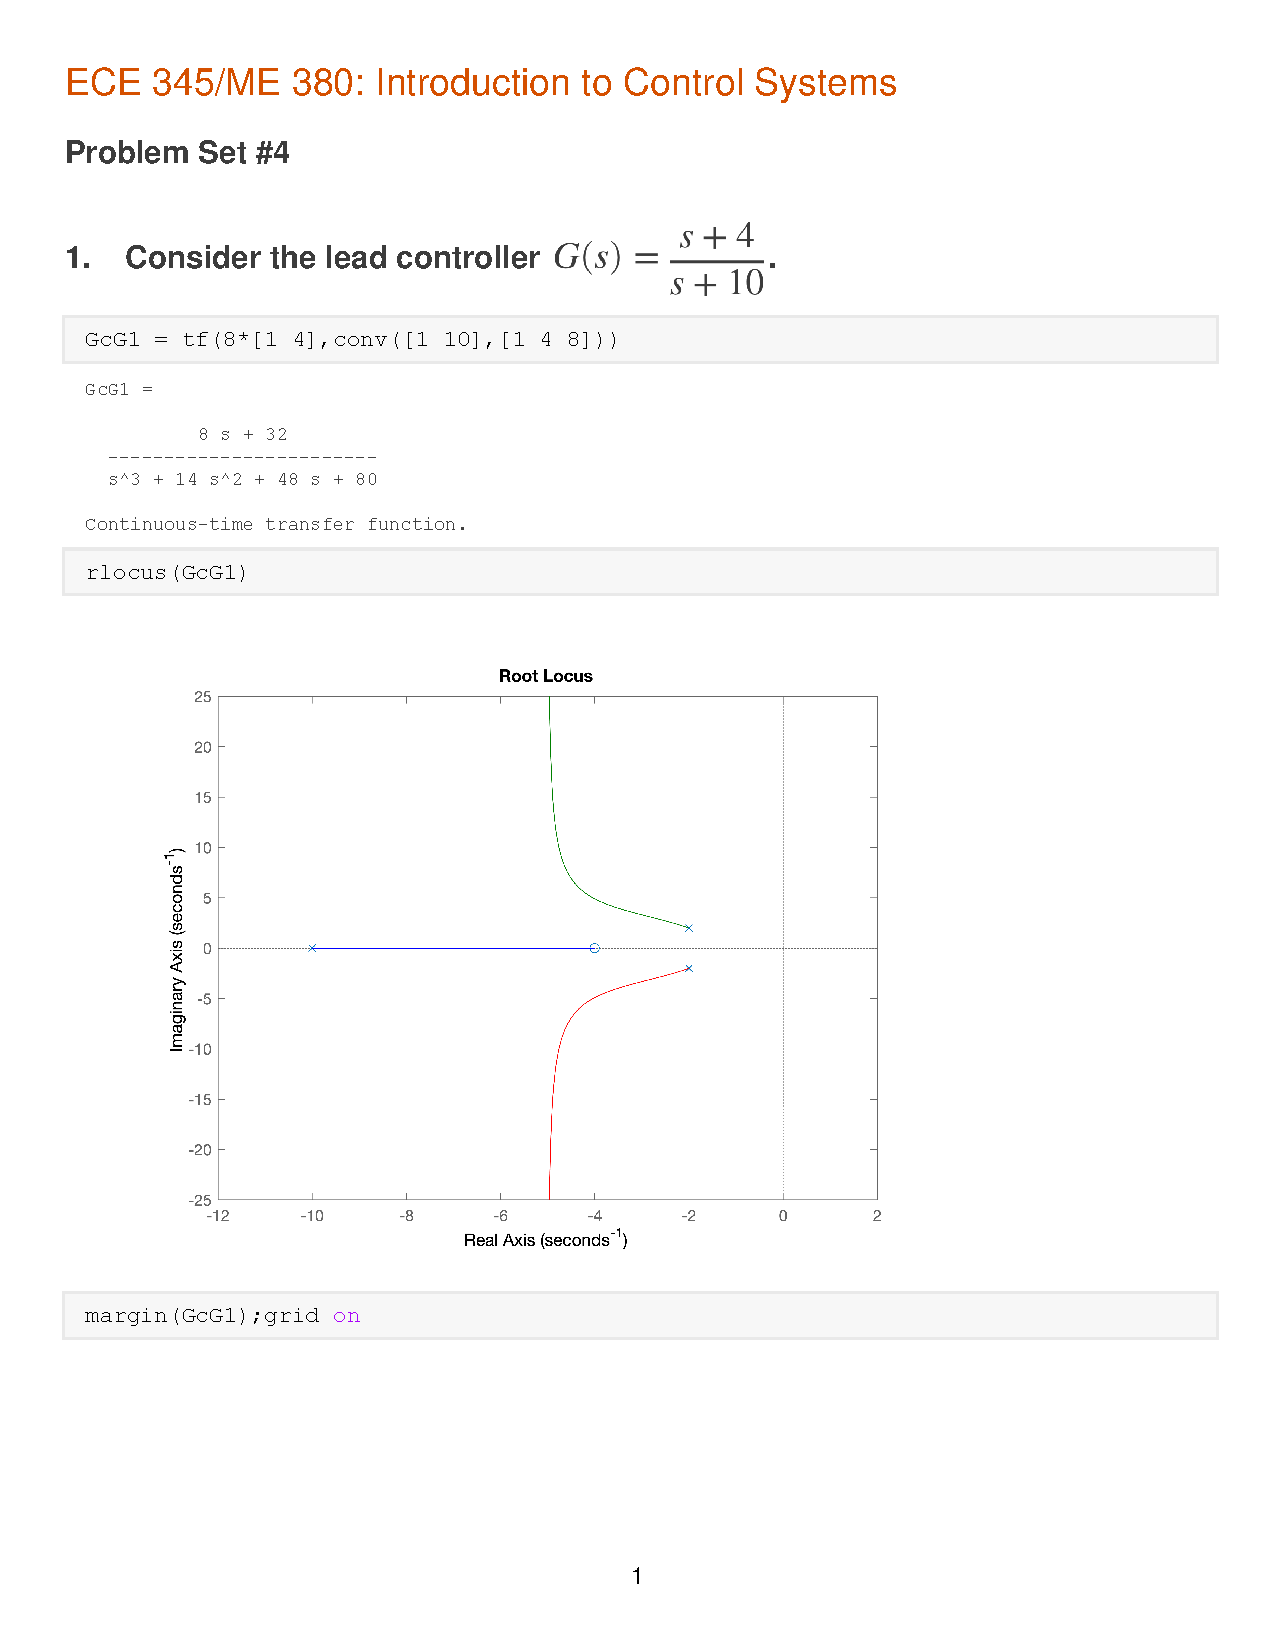
\includepdf[pages=-]{PS4_Matlab.pdf}
\end{document}